%------------------------------------------------------------------------------------
%	PACKAGES AND OTHER DOCUMENT CONFIGURATIONS
%------------------------------------------------------------------------------------

\documentclass{article}

\usepackage{fancyhdr} % Required for custom headers
\usepackage{lastpage} % Required to determine the last page for the footer
\usepackage{extramarks} % Required for headers and footers
\usepackage[usenames,dvipsnames]{color} % Required for custom colors
\usepackage{graphicx} % Required to insert images
\usepackage{subcaption}
\usepackage{listings} % Required for insertion of code
\usepackage{courier} % Required for the courier font
% Optional Packages
\usepackage{amsmath}
\usepackage{amssymb}
\usepackage{float}
\usepackage{algorithm}
\usepackage[noend]{algpseudocode}


% Margins
\topmargin=-0.45in
\evensidemargin=0in
\oddsidemargin=0in
\textwidth=6.5in
\textheight=9.0in
\headsep=0.25in

\linespread{1.1} % Line spacing

% Set up the header and footer
\pagestyle{fancy}
\lhead{\hmwkAuthorName} % Top left header
\chead{\hmwkClass\ : \hmwkTitle} % Top center head
%\rhead{\firstxmark} % Top right header
\lfoot{\lastxmark} % Bottom left footer
\cfoot{} % Bottom center footer
\rfoot{Page\ \thepage\ of\ \protect\pageref{LastPage}} % Bottom right footer
\renewcommand\headrulewidth{0.4pt} % Size of the header rule
\renewcommand\footrulewidth{0.4pt} % Size of the footer rule

\setlength\parindent{0pt} % Removes all indentation from paragraphs


%------------------------------------------------------------------------------------
%	DOCUMENT STRUCTURE COMMANDS
%	Skip this unless you know what you're doing
%------------------------------------------------------------------------------------

% Header and footer for when a page split occurs within a problem environment
\newcommand{\enterProblemHeader}[1]{
	%\nobreak\extramarks{#1}{#1 continued on next page\ldots}\nobreak
	%\nobreak\extramarks{#1 (continued)}{#1 continued on next page\ldots}\nobreak
}

% Header and footer for when a page split occurs between problem environments
\newcommand{\exitProblemHeader}[1]{
	%\nobreak\extramarks{#1 (continued)}{#1 continued on next page\ldots}\nobreak
	%\nobreak\extramarks{#1}{}\nobreak
}

\setcounter{secnumdepth}{0} % Removes default section numbers
\newcounter{homeworkProblemCounter} % Creates a counter to keep track of the number of problems
\setcounter{homeworkProblemCounter}{0}

\newcommand{\homeworkProblemName}{}
\newenvironment{homeworkProblem}[1][Problem \arabic{homeworkProblemCounter}]{ % Makes a new environment called homeworkProblem which takes 1 argument (custom name) but the default is "Problem #"
	\stepcounter{homeworkProblemCounter} % Increase counter for number of problems
	\renewcommand{\homeworkProblemName}{#1} % Assign \homeworkProblemName the name of the problem
	\section{\homeworkProblemName} % Make a section in the document with the custom problem count
	\enterProblemHeader{\homeworkProblemName} % Header and footer within the environment
}{
	\exitProblemHeader{\homeworkProblemName} % Header and footer after the environment
}

\newcommand{\problemAnswer}[1]{ % Defines the problem answer command with the content as the only argument
	\noindent\framebox[\columnwidth][c]{\begin{minipage}{0.98\columnwidth}#1\end{minipage}} % Makes the box around the problem answer and puts the content inside
}

\newcommand{\homeworkSectionName}{}
\newenvironment{homeworkSection}[1]{ % New environment for sections within homework problems, takes 1 argument - the name of the section
	\renewcommand{\homeworkSectionName}{#1} % Assign \homeworkSectionName to the name of the section from the environment argument
	\subsection{\homeworkSectionName} % Make a subsection with the custom name of the subsection
	\enterProblemHeader{\homeworkProblemName\ [\homeworkSectionName]} % Header and footer within the environment
}{
	\enterProblemHeader{\homeworkProblemName} % Header and footer after the environment
}


%=================================================================

%------------------------------------------------------------------------------------
%	NAME AND CLASS SECTION
%------------------------------------------------------------------------------------

\newcommand{\hmwkTitle}{Assignment\ \#4} % Assignment title
\newcommand{\hmwkClass}{CSC 411} % Course/class
\newcommand{\hmwkAuthorName}{Xiangyu Kong \hspace{3em} Yun Lu} % Your name
\newcommand{\hmwkUTorId}{kongxi16 \hspace{5em} luyun5} % UTorID

%------------------------------------------------------------------------------------
%	TITLE PAGE
%------------------------------------------------------------------------------------

\title{
	\vspace{2in}
	\textmd{\textbf{\hmwkClass:\ \hmwkTitle}}\\
	%	\normalsize\vspace{0.1in}\small{Due\ on\ \hmwkDueDate}\\
	\vspace{0.1in}
	\vspace{3in}
}

\author{\textbf{\hmwkAuthorName} \\ \textbf{\hmwkUTorId}}

% Insert date here if you want it to appear below your name
\date{\today}

%------------------------------------------------------------------------------------

\begin{document}
	
	\maketitle
	\clearpage
	
	%---------------------------------------------------------------------------------
	%	PROBLEM 1
	%---------------------------------------------------------------------------------
	\begin{homeworkProblem}
		%		\noindent \textit{Question}
		In class ``Environment", the ``grid" is represented by an 1-D array of 9 elements. Attribute ``turn" represents whose turn it is. The valid values for ``turn" is either 1 (x) or 2 (o). Attribute ``done" represents whether the game is done.
		
		The code and output of a game is shown in the listing below.
		
		\begin{lstlisting}[caption = Code and Output of a game]
		for i in range(9):
			env.step(i)
			env.render()
		return
		x..
		...
		...
		====
		xo.
		...
		...
		====
		xox
		...
		...
		====
		xox
		o..
		...
		====
		xox
		ox.
		...
		====
		xox
		oxo
		...
		====
		xox
		oxo
		x..
		====
		xox
		oxo
		x..
		====
		xox
		oxo
		x..
		====
		\end{lstlisting}
		
	\end{homeworkProblem}
	\clearpage
	
	%----------------------------------------------------------------------------------
	
	
	%---------------------------------------------------------------------------------
	%	PROBLEM 2
	%---------------------------------------------------------------------------------
	\begin{homeworkProblem}

		\begin{enumerate}
			\item 
			The Policy class is implemented in the listing below. The network consist of one hidden layer and the activations used are ReLU activation.
			\begin{lstlisting}[language = python, caption = policy]
class Policy(nn.Module):
	def __init__(self, input_size=27, hidden_size=64, output_size=9):
		super(Policy, self).__init__()
		self.network = nn.Sequential(
			nn.Linear(input_size, hidden_size),
			nn.ReLU(),
			nn.Linear(hidden_size, output_size),
			nn.ReLU())
	def forward(self, x):
		return self.network(x)
			\end{lstlisting}
			
			\item 
			The 27-dimensional vector should be viewed as a $3 \times 9$ matrices with each column as a one-hot vector. The column number represents the position on the grid (1st column represent Environment.grid[0]), and the vector itself represents the state of the current position. The state correspond to the map in Environment.render() (\{0: '.', 1: 'x', 2: 'o'\}).
			
			\item 
			The 9 values Policy returns are the probabilities that it chooses the corresponding next move (e.g. the first element represents the probability that the next move is chosen to be placed at the first element in Environment.grid).
			
			The select\_action samples the action according to the probabilities (stochastic) instead of choosing the maximum probability (deterministic). Then the policy is stochastic.
			
		\end{enumerate}
		
		
	\end{homeworkProblem}
	\clearpage
	
	%----------------------------------------------------------------------------------
	
	
	%---------------------------------------------------------------------------------
	%	PROBLEM 3
	%---------------------------------------------------------------------------------
	\begin{homeworkProblem}
		%		\noindent \textit{Question}
		\begin{enumerate}
			\item 
			the implementation for compute\_returns is shown in the listing below.
			\begin{lstlisting}[language = python, caption = compute return]
def compute_returns(rewards, gamma = 1.0):
	res = []
	for i in range(len(rewards)):
		curr_return = 0
		cur_rewards = rewards[i:]
		for j in range(len(cur_rewards)):
			curr_return += cur_rewards[j] * (gamma ** j)
		res.append(curr_return)
	return res
			\end{lstlisting}
			
			\item 
			The backward pass cannot be computed during the episode because the reward is not fully recorded and thus computing the gradient may produce a biased return.
			
		\end{enumerate}
		
	\end{homeworkProblem}
	\clearpage
	
	%----------------------------------------------------------------------------------
	
	
	%---------------------------------------------------------------------------------
	%	PROBLEM 4
	%---------------------------------------------------------------------------------
	\begin{homeworkProblem}
		%		\noindent \textit{Question}
		\begin{enumerate}
			\item 
			See tictactoe.py for implementations.
			
			\item 
			The rewards are shown in the listing below.
			
			\begin{lstlisting}[caption = Rewards]
	Environment.STATUS_VALID_MOVE: 1,
	Environment.STATUS_INVALID_MOVE: -1,
	Environment.STATUS_WIN: 10,
	Environment.STATUS_TIE: 0,
	Environment.STATUS_LOSE: -10
			\end{lstlisting}
		\end{enumerate}
		
	\end{homeworkProblem}
	\clearpage
	
	%----------------------------------------------------------------------------------
	
	
	%---------------------------------------------------------------------------------
	%	PROBLEM 5
	%---------------------------------------------------------------------------------
	\begin{homeworkProblem}
		%		\noindent \textit{Question}
		\begin{enumerate}
			\item 
			The training curve is shown in Fig.\ref{fig:5}. The hyperparameters are as follows: lr = 0.001, gamma = 1.0, max\_iter = 1000
		
			\begin{figure}[!ht]
				\centering
				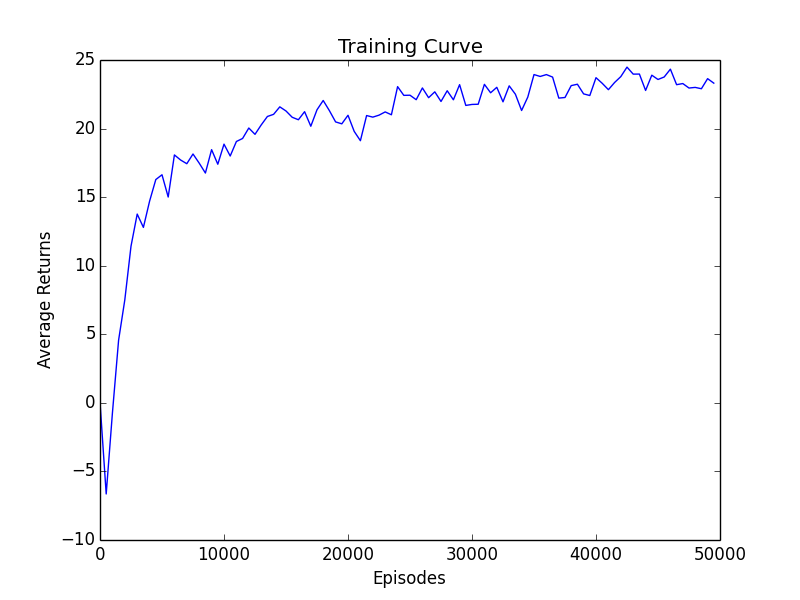
\includegraphics[width=.35\linewidth]{images/5/training_curve.png}
				\caption{caption}
				\label{fig:5}
			\end{figure}
			
			\item 
			
			
			\item 
			
			
			\item 
		\end{enumerate}
		
	\end{homeworkProblem}
	\clearpage
	
	%----------------------------------------------------------------------------------
	
	
	%---------------------------------------------------------------------------------
	%	PROBLEM 6
	%---------------------------------------------------------------------------------
	\begin{homeworkProblem}
		%		\noindent \textit{Question}
		
		
	\end{homeworkProblem}
	\clearpage
	
	%----------------------------------------------------------------------------------
	
	
	%---------------------------------------------------------------------------------
	%	PROBLEM 7
	%---------------------------------------------------------------------------------
	\begin{homeworkProblem}
		%		\noindent \textit{Question}
		
		
	\end{homeworkProblem}
	\clearpage
	
	%----------------------------------------------------------------------------------
	
	
	%---------------------------------------------------------------------------------
	%	PROBLEM 8
	%---------------------------------------------------------------------------------
	\begin{homeworkProblem}
		%		\noindent \textit{Question}
		
		
	\end{homeworkProblem}
	\clearpage
	
	%----------------------------------------------------------------------------------
	
	%---------------------------------------------------------------------------------
\end{document}